
\chapter{Background}
\label{sec:background}
To begin, we introduce some terminology and background information to be used in the chapters to follow.

\section{Reo}
\label{sec:reo_background}
Reo is a high-level language for specifying protocols. In this section, we touch on the motivation behind Reo's development, and explain how it is used. The language has applicability whenever there is a benefit in being able to formalize a communication protocol. However, this work primarily focuses on Reo's role in automatic generation of glue-code for coordinating interactions within executable programs.  

\subsection{Motivation and Purpose}
\label{sec:reo_motivation}
Traditionally, coordination programming is approached much like sequential programming, by laying out program logic as sequences of actions, tracing the path of one control-flow at a time. In such programs, concurrency and parallelism are emergent properties; interactions are not represented explicitly, instead they must be derived from actions sprinkled throughout the program~\cite{arbab2011puff}. The more complex the program, the more difficult it is for programmers to make sense of this coordination; actions that contribute to interactions become entangled with local computation. Depending on the language, there may also be a large conceptual gap between the coordination's underlying concept and the granular operations the program uses to implement it. The larger the gap, the more tightly-integrated they become, obfuscating the concept within implementation specifics and making it difficult to change one without changing the other.

Over time, various tools and languages have emerged, each with their own way to raise the level of abstraction. For example, various process calculi can represent coordination actions symbolically, such that it is more easily understood and manipulated by humans and machines alike~\cite{arbab2011puff}. Chapel is an example of a general-purpose programming language with a focus on parallelism, offering a (more traditional) `local view' mode for concurrent procedures, but also a `global view' mode for data-parallelism that reads much like a sequential program~\cite{chamberlain2007parallel}.
\textit{Coordination languages} are primarily oriented toward expressing the means by which concurrent systems coordinate the actions of individual actors into interactions. Their domain-specific nature often makes them suitable for augmenting other general-purpose languages by increasing their expressive power. \textit{Linda} is said to be the first of its kind~\cite{wells2005coordination}. In Linda, communication between actors takes the form of simple manipulations of tuples in a global value store it calls the \textit{tuple space}. Programmers can thereby separate their concerns of \textit{what} coordination logic is implemented from \textit{how} it is implemented~\cite{gelernter1992coordination}.

Reo is a coordination language founded by the Formal Methods group at the CWI in Amsterdam. It has much in common with Linda, but attempts to do away with what it considers to be a vestige of the world of sequential programming: \textit{action-centricism}, making explicit only individual actions, relegating interactions to a derived concept. Reo represents a program's coordination logic in terms of interactions between participants explicitly; actions of participants can be derived later~\cite{arbab2011puff}. As with Linda, Reo is a domain-specific language, able to take over only the coordination work of a program written in another language. Where Linda embeds tuple operations into its host language, Reo embeds ports; program logic is interspersed with (logical) message-passing port operations. Unlike their Linda equivalents, ports are local structures which are entirely oblivious to their environment, exchanging data with an unknown peer in an unknown system context. Actions serve only to drive local computation tasks. Building a complex system is a matter of \textit{composing} these modular \textit{components} by interfacing their ports. Reo's main purpose is to provide an interaction-centric, declarative language for the specification of a protocol component which acts as an intermediary between other components in the system. The \textit{Reo compiler} sees to the translation from the Reo specification to the equivalent executable code in the target language~\cite{arbab2011puff}.

Reo's approach to programming comes with two advantages: (1)~Programmers may view and manipulate the coordination logic of their program via the Reo specification, whose nature is well suited for tasks such as verification, and (2)~protocol and compute components are loosely coupled to their environment, making it possible to reuse them in different programs, and to understand or alter their behavior in isolation.


\subsection{Language}
\label{sec:reo_lang}
Reo is a graphical language which represents a protocol as a \textit{connector}, a multigraph which defines the relationships between its nodes~\cite{arbab2011puff}. Nodes represent logical `locations' which may observe a single datum at a time. Ultimately, a connector's relations boil down to Reo's underlying semantics, of which there are several to choose from (explained in Section~\ref{sec:semantic_models} to follow). They have in common that they constrain the synchronous observations of data at nodes. For example, a connector may enforce that nodes~$A$ and~$B$ always observe the same data element. This is known as the $sync$ channel, a primitive sufficiently ubiquitous to be represented simply as an arrow ($\longrightarrow$) in Reo's graphical syntax. In this fashion, a connector specifies the ways in which data is permitted to synchronously `flow' through its 	nodes. The literature often uses terms such as `circuit'  to evoke appropriate metaphors. As with electricity or fluid pressure, flow propagates forwards, and blockages propagate backwards.

A tenet of Reo's design philosophy is compositionality (and consequently, modularity). Rather than defining each and every connector anew in terms of the underlying semantics, all but the simplest primitive connectors are built from the composition of others~\cite{arbab2011puff}. At each level of this hierarchy, the connector exposes a subset of its nodes to the connector above, wherein they are called \textit{ports}. The set of a connector's ports is called its \textit{interface}, beyond which is its \textit{environment}. A connector with complex semantics emerges when the ports of its constituent connectors are linked together. 

As Reo's various metaphors suggest, we usually think of data as flowing in a particular direction. To this end, ports are usually defined along with an annotation of their \textit{orientation}: \textit{input} ports accept data from the environment (moving downward in the connector hierarchry), and \textit{output} ports are the reverse. With these orientations, port interactions orient the direction of their flow from \textit{source} nodes to \textit{sinks}. Connectors can define internal nodes of \textit{mixed} orientation by sources to sinks in various configurations. In this way, connectors can specify complex relationships in their \textit{hidden} (internal) nodes. 

Some Reo primitives (and consequently, some connectors that incorporate them) define relationships in terms of variables whose states can persist into the future. In this way, Reo can model asynchronous data flow also, breaking up contiguous networks of synchrony, and constraining future observations in terms of its changing state. The primitive $fifo1$ connector is canonical for this purpose; in observing some datum~$X$ on its single input port, an empty connector becomes full, whereafter the next observation on its single output port must be~$X$, making it empty once again. Despite its simplicity, $fifo1$ is sufficient for the expression of arbitrary asynchronous events and for encoding the persistence of any state.\footnote{The initially-full variant of $fifo1$ allows Reo to express connectors initialized with any imaginable initial state.} These memory variables is explored further in Section~\ref{sec:semantic_models} to follow.

Conventionally, Reo is expressed using graphical syntax, representing nodes as one would expect. Building a connector graphically involves drawing connections between nodes as edges for the usual binary primitives ($sync$, $fifo1$, etc.), or as `black boxes', exposing ports at their boundaries. In this work, we focus on Reo's textual syntax~\cite{dokter2018treo} instead, as it makes for a more practical interface between human and compiler. In this context, the language is fundamentally the same, but relies on textual identifiers for nodes and connectors as is typical for general-purpose programming languages. Listing~\ref{fig:alternator2_spec} demonstrates both methods using a canonical example connector:~$alternator2$.

More complete descriptions of how Reo works, how its nodes behave under composition and details about the canonical Reo primitive connectors are available elsewhere~\cite{arbab2004modeling, arbab2005abstract, arbab2011puff}.



\begin{figure}[htbp]
	\begin{tabular}{p{0.5\textwidth}p{0.5\textwidth}}
		\begin{minipage}{.5\textwidth}
			\centering
			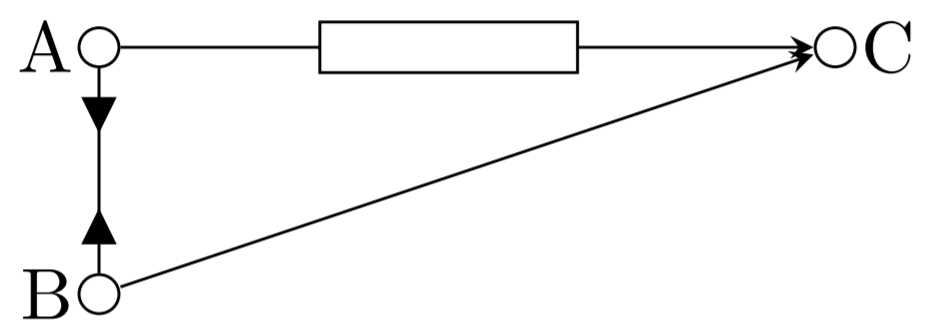
\includegraphics[width=0.80\textwidth]{alt_circ.png}
		\end{minipage}
		&
		\begin{minipage}{.5\textwidth}
			\inputminted{lisp}{alternator2.treo}
		\end{minipage}
	\end{tabular}
	\caption[Graphical and textual specification example.]{Reo specification of the $alternator2$ connector with input ports~$\{A,B\}$, and output port~$C$ using graphical and textual syntax. 
		Data flows to~$C$ from~$A$ and~$B$ in an alternating fashion. Connector is distinct from a $sequencer$ by $B$'s transmission being synchronous with all three ports.
		Figure is taken from~\cite{zhang2019reasoning}.
	}
	\label{fig:alternator2_spec}
\end{figure}

\subsection{Semantic Models}
\label{sec:semantic_models}
Reo took a number of years to take its present shape. It is recognizable as early as 2001, but was presented as a concept before it was formalized, leaving it as a task for future work~\cite{jongmans2012overview}. Later, This several different approaches to formal semantics were developed. For our purposes, it suffices to concentrate only on the small subset of the semantics to follow. For additional information, the work of Jongmans et a.\ in particular serves as a good entry point~\cite{jongmans2012overview}.


Starting with the fundamentals, a \textbf{stream} specifies the value of a variable from data domain $D$ changing over the course of a sequence of events. Usually streams are considered infinite, and so it is practical to define them as a function $\mathbb{N}\mapsto{}D$. A \textbf{timed data stream} (TDS) takes this notion a step further, annotating each event in the sequence with an increasing \textit{time stamp}. A TDS is defined by some tuple $(\mathbb{N}\mapsto{}\mathbb{R}, \mathbb{N}\mapsto{}D)$, or equivalently, $\mathbb{N}\mapsto{}(\mathbb{R}, D)$, with the requirement that time stamps must increase toward infinity~\cite{arbab2004modeling}. By associating one TDS with each named variable of a program, one can represent a trace of its execution. TDS events with the same time stamp are considered simultaneous, allowing reasoning about snapshots of the program's state over its run time. These traces can be practically visualized as \textbf{trace tables}, with variables for columns and time stamps for rows by representing the absence of data observations using a special `silent' symbol \textbf{*}, referring to \textit{silent behavior}. In this work, we introduce \textit{trace tables} as a term for both the tabular visualization, and to a program trace as a set of named TDS's. The runs of finite programs can be simulated either by bounding the tables (constraining the TDS domain to be finite), or by simulating finite behavior as infinite by extending the `end' forevermore with silent behavior. Table~\ref{tab:fifo1_eg} gives an example of a trace table for some program with two named variables.


\begin{table}[]
	\centering
	\begin{tabular}{l|cc}
		$\mathbb{R}$  & A & B \\ \hline
		0.0 & 0 & * \\
		0.1 & * & 0 \\
		0.2 & * & * \\
		0.3 & 1 & * \\
		0.4 & * & 1
	\end{tabular}
	\caption[Trace table of a system adherent to fifo1.]{Trace table comprised of TDS's for variables $A$ and $B$. This trace represents behavior that adheres to the $fifo1$ protocol with input and output ports $A$ and $B$ respectively.}
	\label{tab:fifo1_eg}
\end{table}


One of it's earlier coalegebraic models represented Reo connectors as \textbf{stream constraints} (SC) over such TDS tables in which variables are ports~\cite{arbab2004reo}. Here, constraints are usually defined in first-order temporal logic, which allows the discrimination of streams according to their values both now and arbitrarily far into the future.\footnote{Not all variants of temporal logic are equally (succinctly) expressive. It requires a notion of `bounded lookahead' to express a notion such as `$P$ holds for the next 3 states' as something like $\square ^{1-3} P$ rather than the verbose $(\square P \wedge \square \square P \wedge \square \square \square P)$.} This model is well suited for translating from the kinds of safety properties that are typically desired in practice. Statements such as `$A$ never receives a message before $B$ has communicated with $C$' have clear mappings to temporal logic, as often it is intuitive to reason about safety by reasoning about future events. Table~\ref{tab:fifo1_eg} above shows the trace of a program that adheres the $fifo1$ protocol with ports $A$ and $B$ as input and output respectively.

SC are unwieldy in the context of code generation. In reality, it is easier to predicate one's next actions as a function of the past rather than the future. Accordingly, \textbf{constraint automata} (CA) was one of the operational models for modeling Reo connectors that has a clearer correspondence to stateful computation. Where an NFA accepts finite strings, a CA accepts trace tables. Thus, each CA represents some protocol. Programs are adherent to the protocol if and only if it always generates only accepted trace tables. From an implementation perspective, CA can be thought to enumerate precisely the actions which are allowed at ports given the correct states, and prohibiting everything else by default. A CA is defined with a state set and initial state as usual, but each transition is given \textit{constraints} that prevent their firing unless satisfied; each transition has both (a) the \textit{synchronization constraint}, the set of ports which perform actions, and (b) a \textit{data constraint} predicate over the values of ports in the firing set at the `current' time step. For example, Listing~\ref{tab:fifo1_eg} above is accepted by the CA of the $fifo1$ connector with all ports of binary data type $\{0,1\}$. Observe that here the automaton discriminates the previously-buffered value (`remembering' what $A$ stored) by distinguishing the options with states $q_{f0}$ and $q_{f1}$. As a consequence, it is not possible to represent a $fifo1$ protocol for an infinite data domain without requiring infinite states.
\begin{figure}[ht]
	\centering
	\begin{tikzpicture}
	\node[state, initial above] (q0) {$q_{e}$};
	\node[state, left of=q0] (q1) {$q_{f0}$};
	\node[state, right of=q0] (q2) {$q_{f1}$};
	\draw
	(q0) edge[bend left, below] node{$\{A\}$\\$d_A$=0} (q1)
	(q1) edge[bend left, above] node{$\{B\}$\\\hspace{1em}$d_B$=0} (q0)
	
	(q0) edge[bend right, below] node{$\{A\}$\\$d_A$=1} (q2)
	(q2) edge[bend right, above] node{$\{B\}$\\\hspace{1em}$d_B$=1} (q0)
	;
	\end{tikzpicture}
	\caption[CA for fifo1 connector.]{CA for the $fifo1$ protocol with ports $A$ and $B$ sharing data domain $\{0,1\}$.}
	\label{fig:fifo1_ca}
\end{figure}

Later, CA were extended to include \textit{memory cells} (or \textit{memory variables}) which act as value stores whose contents persist into the future. Data constraints are provided the ability to assign to their next value, typically using syntax from temporal logic (eg: $m'$ is the value of $m$ at the next time stamp)~\cite{arbab2007models}. Figure~\ref{fig:fifo1_ca_mem} revisits the $fifo1$ protocol from before. With this extension, the task of persistently storing $A$'s value into the buffer can be relegated to $m$, simplifying the state space significantly. This change also makes it possible to represent connectors for arbitrary data domains, finite or otherwise.



\begin{figure}[ht]
	\centering
	\begin{tikzpicture}
	\node[state, initial] (q0) {$q_{e}$};
	\node[state, right of=q0] (q1) {$q_{f}$};
	\draw
	(q0) edge[bend left, above] node{$\{A\}$\\$d_A=m'$} (q1)
	(q1) edge[bend left, below] node{$\{B\}$\\$d_B=m$} (q0)
	;
	\end{tikzpicture}
	\caption[CA with memory for fifo1 connector.]{CA with memory cell~$m$ for Reo connector~$fifo1$ with arbitrary data domain~$D$ common to ports~$A$ and~$B$. Two states are used to track to enforce alternation between filling and emptying~$m$.}
	\label{fig:fifo1_ca_mem}
\end{figure}


For the purposes of Reo, we are interested in being able to compute the composition of CAs to acquire a model for the compositions of their protocols. Figure~\ref{fig:fifo2_ca} shows an example of such a composition, producing $fifo2$ by composing $fifo1$ with itself. This new protocol indeed exhibits the desired behavior; the memory cells are able to store up to two elements at a time, and $B$ is guaranteed to consume values in the order that $A$ produced them. Even at this small scale, we see how the composition of such CA have a tendency to result in an explosion if state and transition spaces. When seen at larger scales, a $fifoN$ buffer consists of $2^N$ states. The problem is the inability for a CA to perform any meaningful $abstraction$; here, it manifests as the automaton having to express its transition system in undesired specificity. Intuitively, the contents of $m_0$ are irrelevant when $m_1$ is drained by $B$, but the CA requires two transitions to cover the possible cases in which this action is available. In the context of accepting existing trace tables, data constraints are evaluated predictably. However, in the case of code generation we are able to treat the data constraint instead as a pair of (a) the \textit{guard} which enables the transition as a function of the present time stamp, and (b) the \textit{assignment}, which may reason about the next time step, and which we are able to guarantee by assigning variables. As such, data constraints are broken up into these parts where possible. Figure~\ref{fig:fifo2_ca} and others to follow formulate their data constraints such that the guard and assignment parts are identifiable wherever it is practical to do so.


\begin{figure}[ht]
	\centering
	\begin{tikzpicture}
	\node[state, initial]      (qee) {$q_{ee}$};
	\node[state, right of=qee] (qfe) {$q_{fe}$};
	\node[state, below of=qfe] (qff) {$q_{ff}$};
	\node[state, below of=qee] (qef) {$q_{ef}$};
	\draw
	(qee) edge[above] node{$\{A\}$\\$m_0'=d_A$} (qfe)
	(qfe) edge[below] node[pos=0.43]{$\quad{}\{\}$\\$\quad{}m_1'=m_0$} (qef)
	(qff) edge[right] node{$\{B\}$\\$d_B=m_1$} (qfe)
	(qef) edge[below] node{$\{A\}$\\$m_0'=d_A$} (qff)
	(qef) edge[left] node{$\{B\}$\\$d_B=m_1$} (qee)
	;
	\end{tikzpicture}
	\caption[CA with memory for fifo2 connector.]{CA with memory cells $m_0$ and $m_1$ for the $fifo2$ connector with an arbitrary data domain for ports $A$ and $B$. Transitions are spread over the state space such that the automaton's structure results in the `first-in, first-out' behavior of the memory cells in series.}
	\label{fig:fifo2_ca}
\end{figure}


\begin{figure}[ht]
	\centering
	\begin{tikzpicture}
	\node[state, initial] (q0) {$ $};
	\draw
	(q0) edge[loop above] node{$\{A\}$\\$m=*$\\$\gapwedge{}m'=d_A$} (q0)
	(q0) edge[loop below] node{$\{B\}$\\$m\neq{}*$\\$\gapwedge{}d_B=m\gapwedge{}m'=*$} (q0)
	;
	\end{tikzpicture}
	\caption[RBA for fifo1 connector.]{RBA of the $fifo1$ connector for an arbitrary data domain common to ports $A$ and $B$. Memory cell $m$ is used both to buffer $A$'s value, and as part of the data constraint on both transitions for emptying and filling the cell to ensure these interactions are always interleaved. Data constraints are formulated for readability such that the `guard' and `assignment' conjuncts are line-separated.}
	\label{fig:fifo1_rba}
\end{figure}
Evidently, memory cells provide a new means of enforcing how data persists over time. In many cases, it can be seen that the same connectors can be represented differently by moving this responsibility between state and data domains. \textbf{Rule-based automata} (RBA) are the cases of CA for which this idea is taken to an extreme by relying only on memory cells entirely; RBAs have only one state~\cite{dokter2018rule}. Figure~\ref{fig:fifo1_rba} models the $fifo1$ connector once again, this time as an RBA. Aside from the added expressiveness, RBAs benefit from being cheaper to compose. As the state space is degenerate, RBAs may be easily reinterpreted into forms more easy to work with. \textbf{Rule-based form} (RBF) embraces the statelessness of an RBA as a single formula, the disjunction of its constraints. In this view, Dokter et al.\ defines their composition of connectors such that, instead of exploding, the composed connector has transitions and memory cells that are the sum of its constituent connectors.



\begin{figure}[ht]
	\centering
	\begin{tikzpicture}
	\node[state, initial] (q0) {$ $};
	\draw
	(q0) edge[loop above] node{$\{A\}$\\$m_0=*$\\$\gapwedge{}m_0'=d_A$} (q0)
	(q0) edge[loop right] node{$\{\}$\\$m_0\neq{}*\gapwedge{}m_1=*$\\$\gapwedge{}m_1'=m_0\gapwedge{}m_0'=*$} (q0)
	(q0) edge[loop below] node{$\{B\}$\\$m_1\neq{}*$\\$\gapwedge{}d_B=m_1\gapwedge{}m_1'=*$} (q0)
	;
	\end{tikzpicture}
	\caption[RBA for fifo2 connector.]{RBA of the $fifo2$ connector for an arbitrary data domain common to ports $A$ and $B$. Memory cells $m_0$ and $m_1$ are drained by $B$ in the order they are filled by $A$, and have a capacity of 2 elements. Data constraints are formulated for readability such that the `guard' and `assignment' conjuncts are line-separated.}
	\label{fig:fifo2_rba}
\end{figure}



RBAs have a structure more conducive to simplification of the transition space, such that one RBA transition may represent several transitions in a CA. Figure~\ref{fig:fifo2_rba} shows how how this occurs for the $fifo2$ connector. Where the CA in Figure~\ref{fig:fifo2_ca} must distinguish the cases where $A$ fills $m_0$ as two separate transitions, the RBA is able to use just one; likewise for the transitions representing cases where $B$ is able to drain $m_1$. This `coalescing' of transitions in RBAs is possible owing to the collapsing of their state space. Even without an intuitive understanding of why such transitions can be collapsed, such cases may often be identified only by inspecting the syntax of the data constraints. For another example of CA, a na{\"i}ve translation to RBA might produce two transitions with data constraints $m=*\wedge{}\;X$ and~$m\neq{}*\wedge{}\;X$ for some~$X$, which are both covered by a single data constraint $X$. As both RBA and RBF share this property, we usually refer to RBA transitions and RBF disjuncts as \textit{rules}, giving these models their name. By distinguishing CA transitions from RBA rules in terminology, we are perhaps more cognizant of the latter's increased ability to abstract away needless data constraints. 

\begin{listing}[ht]
	\inputminted[]{java}{putget.java}
	\caption[Type state automaton in Java.]{An example of a program which implements a two-state automaton in the Java programming language. Observe that the behavior of states $A$ and $B$ are encoded implicitly in the structure of the program, while determining which of the two in $A$ are available $A$ requires a check ar runtime.}
	\label{listing:putget}
\end{listing}
Typically, Reo has used the $Data$ domains in both CA and RBA as parallels to the data types of the ports. In most of the languages in which Reo protocols are implemented, the discriminants of such types are not distinguished statically. For example, the C language lacks a way to statically enforce a that function \code{void foo(int x)} is only invoked when $x$ is prime. Instead, checks at runtime are used to specialize behavior. On the other hand, the state space is simple enough to afford a practical translation into the structure of the program itself, requiring no checking at runtime. For example, Listing~\ref{listing:putget} shows an intuitive representation of a connector that alternates between states $A$ and $B$, getting data $x$ from its environment in $A$, and emitting $x$ when $x=3$. Observe that there is no need to protect operations by which state the corresponding CA is in at runtime. This observation has implications for the behavior of implementations of RBAs, as they `cannot remember' which state they are in and must thus perform more checking. In practice, the overhead of this checking is manageable, and does not explode under composition as the state space of CAs tend to do. The representation of automata in programming languages is explored in more detail in Section~\ref{sec:type_state}.

\subsection{The Reo Compiler}
An ecosystem of tooling has emerged around the Reo language, each exploiting Reo's explicit connector specifications for some purpose or another, ranging from verification to code generation. An overview of these tools can be seen on Reo's  website\footnote{\url{http://reo.project.cwi.nl}}. In this work, we are particularly interested in the \textit{Reo compiler}. Previously, code generation was a feature of Reo's \textit{Extensible Coordination Tools} platform plugins for the Eclipse IDE. Since then, the compiler has become a standalone program changing in its design, and being extended to support new compilation targets in response to the developments as the result of ongoing research~\cite{jongmans2012automatic, jongmans2015partially, dokter2018rule}.

Given a textual Reo specification, the Reo compiler generates and emits a \textit{protocol object} with runtime behavior corresponding with the input specification. The output is in a \textit{target language} selected by the user. At time of writing, languages Java, Promela and Maude are supported. C11 is available also, but has been deprecated. Once parsed, the compiler translates the Reo-language representation into that of Rule-based form, involving operations hiding, projection, merging and so on. For our purposes, it suffices to trust that the compiler performs this transformation to our satisfaction, resulting in a representation with the intended semantics. Detailed information about this process is available in the literature~\cite{arbab2004reo, arbab2005abstract, dokter2018rule}. Accordingly, the textual Reo language has support for the definition of primitives in such models directly~\cite{dokter2018treo}. Listing~\ref{listing:fifo1_treo} demonstrates this with the primitive $fifo1$ connector. 


\begin{listing}[ht]
	\inputminted[]{text}{fifo1.rba.treo}
	\caption[Fifo1 connector specfication in textual Reo language.]{Textual Reo specification of the $fifo1$ connector using RBA semantics. Data is asynchronously forwarded from input~$A$ to output~$B$ by being buffered in between in memory cell~$m$.}
	\label{listing:fifo1_treo}
\end{listing}

In this work, we concentrate on Reo's use for the generation of glue code between compute components in a target language, such that the program adheres to the associated Reo specification at runtime. The Reo compiler is responsible for this translation quickly and reliably. Programmers are able to exploit the correspondence between program and specification by using the representation that best fits the task at hand; it runs with all the characteristics of the target language, but programmers may manipulate or verify its coordination properties via its specification.


\section{Target Languages}
In this section we introduce terminology relevant to the languages targeted for code generation by the Reo compiler. We identify patterns and properties that are relied upon in later chapters.

\subsection{Affine Type Systems}
\label{sec:affine_type_systems}
In a nutshell, affine types are characterized by modeling values as finite resources, operations on which \textit{consume} them. This notion of `affinity' has its roots in logic. In a type-theoretic proof system, one can attempt to derive some \textit{judgment} $\Gamma\vdash{}t:\tau$ with \textit{statements} assigning \textit{types} to \textit{terms}; here term~$t$ is stated to have type~$\tau$ under context~$\Gamma$. A context is simply a list of statements, which can be thought to correspond with \textit{assumptions} or \textit{premises}~\cite{nederpelt2014type}. The judgment holds if one can construct a proof, starting with the judgment, selecting and applying \textit{rules} until no `dangling' judgments remain. For example, simply-typed lambda calculus has a type derivation rule for abstraction, substitution and application. Depending on the type system, \textit{structural rules} may additionally be provided for manipulating (`massaging') the context such that other rules may be applied. Consider the following structural rules:

\[
\begin{aligned}
(var): \frac{}{t:\tau \vdash t: \tau}
&\quad
(weaken): \frac{\Gamma \vdash \Sigma}{\Gamma, A \vdash \Sigma}
&\quad
(contract): \frac{\Gamma, A, A \vdash \Sigma}{\Gamma, A \vdash \Sigma}
\end{aligned}
\]

In order of their appearance, $var$ terminates proof branches by identifying tautologies, statements defined directly by the context. $weaken$ allows us to arbitrarily grow our context, weakening the strength of the formula as a whole by adding to our assumptions. $contraction$ allows us to treat statements as if they are idempotent; we are allowed to discard duplicate statements at will. 

Depending on the proof system, such structural rules may be necessary to make a formula provable~\cite{nederpelt2014type}. For example, $weaken$ rule is required to prove $A, t:\tau\vdash t:\tau$. $var$ cannot be directly applied, because $A$ is `in the way'. The set of available rules characterizes the system by determining what can be proven. For example, the ability to arbitrary replicate, discard and rearrange context expressions characterizes a type system whose context is `set-like'; in such a system, the order of statements in the context has no impact on whether a formula can be proven.

Affine type systems are characterized by the absence of $contraction$ rule. Proofs cannot replicate statements at will, and thus they are a finite \textit{resource} in the proof, consumed by use in rules~\cite{walker2005substructural}.

As type systems do in general, type affinity excludes some programs from being expressed. In the context of programming languages, why would we want this? Of course, conventional computer hardware has no problem replicating the bytes representing some integer. Why then do we limit ourselves? This argument can be made for type systems in general; the machine likewise has no problem reinterpreting the bytes storing a string as an integer. This limitation is a feature in and of itself as long as the programs lost are usually somehow `undesirable'. For example, it is exceedingly common practice to dedicate a memory region to one type for the duration of the program, making a case for the feasibility of statically-typed local variables. These reasons are primarily for programmers and not for the program, strictly enforcing what would otherwise be good programming practices. 


\subsection{The Rust Language}
\label{sec:rust_language}
Rust is an imperative, general-purpose, systems programming language most similar to~C++, even (mostly) sharing its C-style syntax. What sets Rust apart is its memory model. Rust is not a memory-managed language, and has no runtime whatsoever. Instead, the language relies on its \textit{ownership system} to predictably insert deallocations (called \code{drop} in Rust) at the right moment such that it runs much as C++ would without exposing these details to the programmer.
To make this possible, the Rust compiler keeps track of the variable binding which \textit{owns} a value at all times. Owned values are affine, and associating them with new variable bindings invalidates their previous binding. In Rust, this is called \textit{moving}, and doubles (at least conceptually) with the relocation of a value in memory. Listing~\ref{listing:move} illustrates how this appears to a programmer; In~\code{main}, the variable~\code{x} is moved into the scope of~\code{func}. The subsequent access of~\code{x} on line~8 is invalid, preventing this program from compiling. Once an owned value goes out of scope, it is no longer accessible, and Rust performs any destruction associated with that type. Along with the RAII (`resource acquisition is initialization') pattern popularized by C++, programmers can rest assured that their resources are created and destroyed on demand, without the need for any bookkeeping at runtime.

\subsubsection{Borrowing}

On their own, movement is incredibly restrictive; there is no apparent way to use any resource without destroying it. To reclaim some vital functionality, Rust has the \textit{borrow system} to facilitate the creation and management of types whose ownership is dependent on others. Similar to those in~C++, programmers are able to create \textit{references} to values (also called `borrows' in Rust terms), which are indistinguishable from pointers at runtime, but have special static semantics. These references are new types, and thus do not represent a transference of ownership to a new binding. Listing~\ref{listing:move2} demonstrates the example from before, but now passing the~\code{x} by reference into \code{func} such that~\code{x} is not invalidated. The Rust compiler's \textit{borrow checker} relies on variable scoping to keep track of these borrows to ensure they do not outlive their referent, as these would manifest at runtime as dangling pointers. This relationship between value and reference is referred to in Rust as the reference's \textit{lifetime}. Rust performs this static analysis at a per-function basis. As such, it is necessary for programmers to fully annotate the input and output types of functions, but they can usually be inferred within function bodies. This has an important consequence; the compiler does cross the boundaries between functions to interpret their relationship. 

For some types there is no practical reason to enforce affinity. This is usually the case for primitives such as integers. For these cases, the language uses the \code{Copy} trait to opt out of Rust's affine management of these resources. Copy-types behave in ways familiar to C and C++ programmers. Listing~\ref{listing:move} from before would compile just fine if Rust's 4 byte unsigned integer type~\code{u32} was used in place of~\code{Foo}.

C and C++ have no inherent support for preventing data races. The programmer is in full control of their resources. It is all too easy to create data races to~C by unintentionally accessing the same resource in parallel precautions. One of the tenets of Rust's design is to use its ownership system to prohibit these data races at compile time. For this reason, Rust has an orthogonal system for \textit{mutability}. References come in two kinds: mutable and immutable. The distinction is made explicit in syntax with the \code{mut} keyword. Rust relies on a simple observation of the common ingredient for all data races: mutable aliasing; only changes to the aliased (one resource accessible by multiple bindings) resource manifest as data races. Rust's approach is thus simply to prohibit mutable aliasing by preventing these conditions from coexisting. Mutable references must be unique (prohibiting aliasing) and immutable references do not allow for any operations that would mutate their referent (prohibiting mutability). This is the same thinking behind the readers-writer pattern for the eponymous lock: there is no race condition if readers coexist, but if one writer exists, it must have exclusive access. 




\begin{listing}[ht]
	\centering
	\inputminted[]{rust}{move.rs}
	\caption[Example of move semantics in Rust.]{Type \code{Foo} is affine. On line 7, $x$ is moved into function \code{func}, consuming it. Accessing $x$ is invalid, and so line 8 raises an error.}
	\label{listing:move}
\end{listing}

\begin{listing}[ht]
	\centering
	\inputminted[]{rust}{move2.rs}
	\caption[Example of borrowing in Rust.]{\code{Foo} is an affine resource. New references to \code{x} are created and sent into code{func} without changing the ownership of \code{x}. Rust's \textbf{borrow checker} ensures that these borrows do not outlive \code{x}.}
	\label{listing:move2}
\end{listing}

\subsubsection{Traits and Polymorphism}
The primary means of polymorphism in Rust is through generic types with \textit{trait bounds}, also called `type parameters'. \textit{Traits} are most similar to interfaces in Java, categorizing a group of instantiable types by defining abstract functions for which implementors provide definitions. Unlike Java, Rust traits say nothing about fields and data, thus describing only their behavior. In this manner, Rust traits are somewhat like C's header files, but rather to be defined per implementor type. Elsewhere in the program, functions and structures can make use of generic types. These types are arbitrary and thus opaque to any behavior save for those common to all Rust types; for example, any type at all can be moved or can be borrowed in Rust. To perform more specialized operations on these generic types, they can be bounded with traits. This acts as a contract between the generic context and its concrete call site; the caller promises that the generic type is reified only with a type which implements the specified traits, and thus the generic can be used in accordance with the behavior these traits provide. This is demonstrated in Listing~\ref{listing:traits}. Here, \code{something} is a function which can be invoked with \code{T} chosen to be any type implementing trait \code{T}, such as \code{String}. 

\begin{listing}[ht]
	\centering
	\inputminted[]{rust}{traits.rs}
	\caption[Generic type example in Rust.]{Definition of a function \code{something} generic over some type \code{T}, where \code{T} implements trait \code{PrintsBool}. Types can implement this trait by providing a definition for all the associated functions, in this case, only \code{print\_bool}.}
	\label{listing:traits}
\end{listing}

Above, we see how a function can be defined such that it operates on a generic type. However, the function cannot be used until the type is chosen concretely for a particular instance. This choice is called \textit{dispatch}, and Rust offers two options: static and dynamic. \textit{Static dispatch} (also called `early binding') is used when the called function can be informed which concrete type has been chosen statically, as the caller knows it at the call-site. During compilation, the generic function is \textit{monomorphized} for the type chosen in this manner on a case-by-case basis, generating binary specialized for that type as if there were no generic at all. Static dispatch is used in C++ templates, and opted-out with the keyword \code{virtual}. This is Rust's second option: \textit{dynamic dispatch} (also called virtual functions or late binding) where the generic function exists as only one instance, and all of the specialized operations on the generic type are resolved to concrete functions at runtime by traversing a layer of indirection: functions are `looked up' in a virtual function table (vtable). Java uses such virtualization extensively, which allows a lot of flexibility such as allowing functions to be overridden by downstream inheritants. Precisely how a language represents virtual functions and lays out the data in memory varies from language to language. Rust uses the \textit{fat pointer} representation for these dynamic objects (also called \textit{trait objects}). Concretely, some generic object which is known only to implement trait~\code{Trait} is represented as a pair of pointers; the first pointing to the actual object' data, and the second pointing to a dense structure of meta-data and function pointers for the methods of~\code{Trait}, usually embedded into the text section of the binary by the Rust compiler itself. Both methods of dispatch are exemplified in Listing~\ref{listing:dispatch}, demonstrating how static dispatch must propagate generics to the caller for resolution to concrete types at compile time, while one function using dynamic dispatch is able to handle any virtualized types by resolving their methods at runtime.


\begin{listing}[ht]
	\centering
	\inputminted{rust}{dispatch.rs}
	\caption[Static vs dynamic dispatch in Rust.]{Static and dynamic dispatch in Rust exemplified. \code{func\_static} shows the former, propagating the type parameter to the caller. \code{func\_dynamic} shows the latter, relying on a virtual function table to resolve the concrete function at runtime. Function \code{main} shows how both appear at the call site.}
	\label{listing:dispatch}
\end{listing}


Rust uses traits for just about everything. Some traits are defined in the standard library, and have a degree of `first class' status by having special meaning when used in combination with the language's syntax. For example,~\code{Not} is a trait that defines a single function,~\code{not}, which is invoked when the type is negated using the usual exclamation syntax, i.e.,\ \code{!true}. Some traits have no associated functions, instead exist for the purpose of communicating information to the compiler. Seen before,~\code{Copy} is a trait which disables the Rust compiler's checks of a value's affinity. \code{Copy}-types may be passed by value. On the other hand, \code{Drop} associates the \code{drop} function with a type, which the compiler will invoke when it goes out of scope; this is the parallel to the definition of destructors in C++. It is common practice in Rust to rely upon common traits such as these for frequently-occurring cases. For example, it is considered good practice to implement \code{Debug} on ones custom traits such that they have a defined means of handling the `debug print' format specifier (e.g.,\ \code{print!("{:?}", foo)}), enabling ones types to be used as a parameter to \code{printf} and so on.

\subsubsection{Enums and Error Handling}
As in C, Rust usually relies on \code{struct} for defining its types. Each is defined as the list of its constituent fields. Creation of these structures necessitates building all of their constituents, and all fields exist at once. By contrast, \textit{sum types} have \textit{variants} only one of which may be present at a time. Arguably, the duck-typing of Python and flexible polymorphism of Java do the work of these sum types; a variable can be bound to anything and then its `variant' can be reflected at runtime using some explicit operations (\code{ininstance} and \code{instanceof} respectively). C takes the approach fitting the language's philosophy; \code{union} types represent any one of its constituents but the program is at the mercy of the programmer to interact with it as the correct variant as they see fit. Rust's solution is similar to C's unions, but its focus on safety required the use of \textit{tags}, an explicit integer to mark the variant to allow for runtime reflection. In Rust, an \code{enum} type is defined with a list of variants, only one of which may exist per intance at a time. At runtime, the variant can be descriminated by explicitly pattern-matching, inspecting some implicit meta-data field of the enum stores to reflect which of the variants is in use. Like C's unions, each variant can be an arbitrary type (another struct for example), these variants can be of heterogeneous size, and thus are represeted by the largest of their variants plus the space for the tag. 

Unlike Java and Python, Rust has no mechanism for \textit{throwables} which override the default control flow, usually for the purposes of ergonomically handling errors. Instead, Rust represents all recoverable errors in the data domain as enums. The standard library defines \code{Option} and \code{Result} enums, which are monadic in that they wrap the `useful' data as one of the variants, but represent the possibility for other variants also. They differ in that \code{Option::None} carries no data, and thus \code{Option} is generic only over one type, the contents of the \code{Some} variant. \code{Result}, on the other hand, has two generic types, one for its `successful' \code{Result::Ok} variant, and one for its `unsuccessful' \code{Result::Err} variant. Listing~\ref{listing:enums} gives an example of typical error-handling in Rust; here, \code{divide\_by} relies on \code{Result} to propagate the error for the caller to handle. In circumstances where the error is unrecoverable, Rust uses a thread \textit{panic}, which unrolls the control flow (printing debugging information if an environment variable is set). This is somewhat similar to Java's \code{Error}.

\begin{listing}[ht]
	\centering
	\inputminted[]{rust}{enums.rs}
	\caption[TODO.]{Demonstrating the Rust idiom of using a \code{Result} in return position to propagate exceptions to the caller for handling. Here, \code{main} must \code{match} the return value to acquire the result contained within the \code{Result::Ok} variant.}
	\label{listing:enums}
\end{listing}

\subsection{The Type-State Pattern}
\label{sec:type_state}

The \textit{state machine} pattern refers to the practice of explicitly checking for or distinguishing transitions between and requirements of states in a stateful object.\footnote{Usually, we ignore program termination. Equivalently, this pattern only allows one to describe automata in which every `useful' state reaches some final `terminated' state.} Usually, these states are distinguished in the data domain of one or more types. Even the lowly \code{Option} type can be viewed as a small state machine as soon as some condition statement specializes operations performed with it. Although its uses are ubiquitous in application development in general, this pattern is particularly useful for those for which the added ability to manage complexity is necessary: video games, for example~\cite{nystrom2014game}.

As the name suggests, the \textit{type state} pattern is an instance of the state pattern, characterized by encoding states as types, which usually are distinct from data in their significance to a language's compiler or interpreter. A common approach is to instantiate one of the state types at a time. Usually, objects with this type do not contain any data at runtime (i.e., they can be represented in memory with zero bytes of field-data). We refer to these objects as \textit{tokens}, suggesting their small size and role as a sort of `currency' in that they are useless in and of themselves, but may be used to facilitate other things.

As an example, consider the scenario where a program wants to facilitate alternation between invoking some functions \code{one} and \code{two} which repeatedly mutate some integer $n$. Listing~\ref{listing:typestateeg} gives an example of what this might look like as a deterministic finite automaton in the C language. In this rendering, the expression \code{two(one(START)).n} evaluates to the expected result of $(0 + 1) \cdot{} 2 = 2$. Even for this simple example, the encoding of states as types in particular has its benefits; the expression \code{one(two(START))} may appear sensible at first glance, but the compiler is quick to identify the type mismatch on the argument to \code{one}, making clear that the expression does not correspond to a path through the automaton:
\begin{verbatim}
note: expected 'DoTwo' but argument is of type 'DoOne'
\end{verbatim}

The type state pattern can be applied in any typed language, but it is particularly meaningful in languages where the compiler or interpreter enforces its intended use. The example above demonstrates some utility, but a language such as C has no fundamental way to prevent the programmer from reusing values. 
If the programmer misbehaves, they can retain their previous states when given new ones, and then invoke the transition operations as they please. It's not much of a state machine if all states coexist, is it? This is not always a problem in examples such as the previous. Here, the types prevent the construction of malformed expressions, and perhaps this is enough. However, we cannot so easily protect a resource from any side effects of \code{one} or \code{two}; imagine the chaos that would result from these functions writing to a persistent file descriptor.
\begin{listing}[ht]
	\inputminted[linenos,tabsize=2,breaklines,frame=lines]{c}{typestate_eg.c}
	\caption[Type state automaton in C with expressions modeling runs.]{An example of the type-state pattern in the C language. The alternating invocation of \code{one} and \code{two} is translated to type checking the compiler can guarantee. This example guarantees that well-formed expressions can be interpreted as valid paths in some corresponding automaton, as the types must match.}
	\label{listing:typestateeg}
\end{listing}

An affine type system overcomes the shortcoming illustrated above. By treating instances of these types as affine resources, the programmer cannot retain old states without violating the affinity of the types. The example looks very similar when translated to Rust, but now a case such as that shown in Listing~\ref{listing:typestateeg2} will result in the compiler preventing the retention of the variable of type \code{DoOne}.

\begin{listing}[ht]
	\inputminted[]{rust}{typestate_eg2.rs}
	\caption[Type state automaton in Rust with execution traces as runs.]{A demonstration of how the type-state encoding shown in Listing~\ref{listing:typestateeg} can leverage affine types to ensure that not only expressions, but a trace through execution can be interpreted as valid paths through some corresponding automaton. The compiler correctly rejects this example, which corresponds with attempting to take transition \code{two} twice in a row.}
	\label{listing:typestateeg2}
\end{listing}

\subsection{Proof-of-Work Pattern}
\label{sec:proof_of_work}
Section~\ref{sec:type_state} demonstrates how the type-state pattern can be used as a tool to constrain actions the compiler will permit the program to do. Indeed, this is a natural parallel to the affinity of the type system, which guarantees that no resource is consumed repeatedly. The counterpart to affine types is \textit{relevant} types, which defines correctness as each resource being consumed at least once. Type systems that are both relevant and affine are \textit{linear}, such that all objects are consumed exactly once.

There is no way to create true relevance or linearity in user space of an arbitrary affine type system; any program which preserves affinity is able to exit at any time without losing affinity. How are we able to enforce a behavior if it is correct to exit at any time? \textit{Proof-of-work} is a special case of the type-state pattern which allows the expression of a relevant type under the assumption that the program continues its normal flow; i.e., system exits are still permitted. The trick to enforcing the use of some object \code{T} is to specify that a type is a function which must return some type \code{R}, and to ensure that \code{R} can only be instantiated by consuming \code{T}. Clearly, we cannot prevent \code{T} from being destroyed in some other way, but we are able to prevent \code{R} from being created any other way.

Realistic languages have many tools for constraining what users may access, such as Java's visibility keywords. Rust has \textit{orphan rules} to prevent imported traits from being implemented for imported types. Languages without any such features won't be able to prevent users from creating the return type \code{R} without consuming \code{T}. In these cases, another option is \textit{generative types} which, among other things, allow us to further distinguish types with different origins. Here, generative types may be used to ensure not just any \code{R} is returned, but a particular \code{R} within our control. As this work uses the Rust language for concrete implementations, we will rely on its ability to prohibit the user from creating \code{R} by using \textit{empty enum types} for types with no data nor type constraints, and by making its fields and constructors with the \textit{private} visibility keyword otherwise\cite{exotic_sizes}.

Consider the following illustrative scenario: We wish to yield control flow to a user-provided function. Within, the user is allowed to do whatever they wish, but we require them to invoke \code{fulfill}  exactly once (which corresponds to `consuming \code{R}'). How can we express this in terms the compiler will enforce? Listing~\ref{listing:promise} demonstrates a possible implementation (omitting all but the essence of `our' side of the implementation). The user's code would then be permitted to invoke \code{main} with their own choice of callback function pointer. Our means of control is the interplay between dictating both (a)
the signature of the callback function and (b) prohibiting the user from constructing or replicating \code{Promise} or \code{Fulfill} objects in their own code.

\begin{listing}[ht]
	\inputminted[]{rust}{promise.rs}
	\caption[Proof of work pattern example of `promises'.]{A demonstration of proof-of-work pattern. Here, the user is able to execute \code{main} with any function as argument, but it must certainly invoke \code{fulfill} exactly once.}
	\label{listing:promise}
\end{listing}
